\PassOptionsToPackage{dvipsnames,table}{xcolor}
\documentclass[10pt]{beamer}
\usepackage{Cours}


\begin{document}

\input{\detokenize{/home/fenarius/Travail/Cours/cpge-info/latex//MacrosCours.tex}}

% Numéro et titre de chapitre
\setcounter{numchap}{4}
\newcommand{\Ctitle}{\cnum $k$ plus proches voisins, $k$ moyennes}

\makess{\textit{knn} : exemple introductif}
\begin{frame}{\Ctitle}{\stitle}
    \begin{exampleblock}{Un champ de fleurs}
        Dans un champ, à l'état sauvage deux types de fleurs ont poussés : des coquelicots et des violettes. On a représenté ci-dessous par un schéma la position de ces fleurs dans le champ
        \begin{center}
            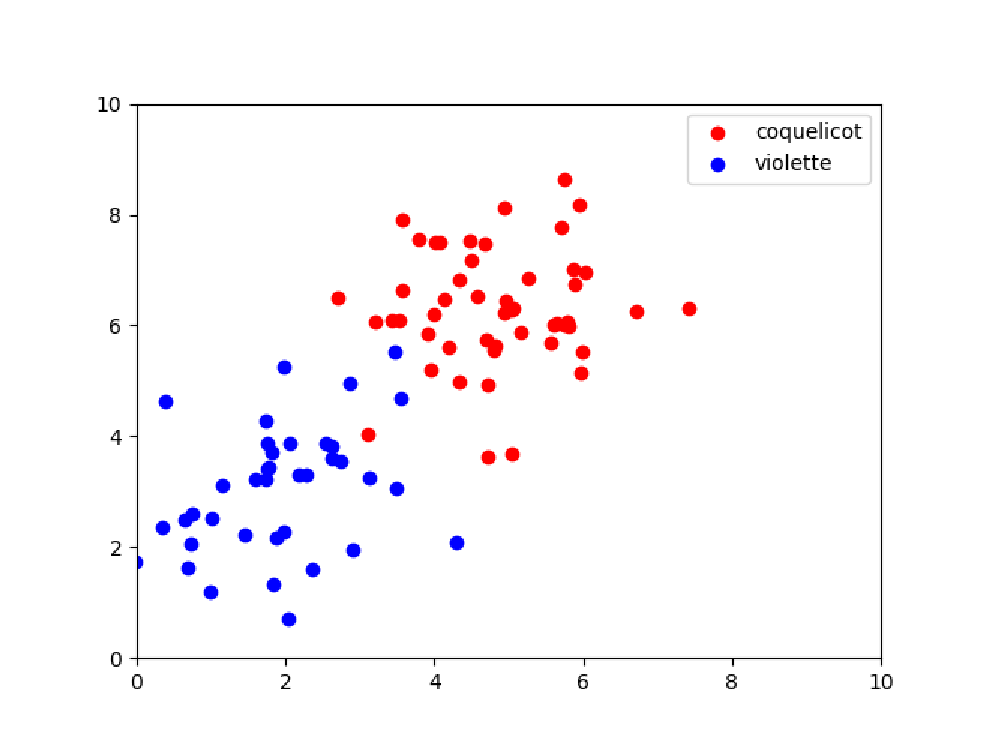
\includegraphics[height=5cm]{ex_cours1.eps}
        \end{center}
    \end{exampleblock}
\end{frame}


\begin{frame}{\Ctitle}{\stitle}
    \begin{exampleblock}{Un champ de fleurs}
        Trois nouvelles pousses, notées $P_1$, $P_2$ et $P_3$ (en gris sur le schéma) font leur apparition. Et on cherche à prédire si ces pousses sont des coquelicots ou des violettes.
        \begin{center}
            \includegraphics[height=5cm]{ex_cours2.eps}
        \end{center}
    \end{exampleblock}
\end{frame}


\begin{frame}{\Ctitle}{\stitle}
    \begin{exampleblock}{Un champ de fleurs}
        On a tracé ci-dessous un cercle de façon apparaître les 5 voisins les plus proches de $P_3$. Choisir l'espèce majoritaire de ce cercle pour classer la nouvelle pousse $P_3$ est un exemple de l'application des $5$ plus proches voisins (\textit{nearest neighbours} en anglais, abrégé en \textit{nn})
        \begin{center}
            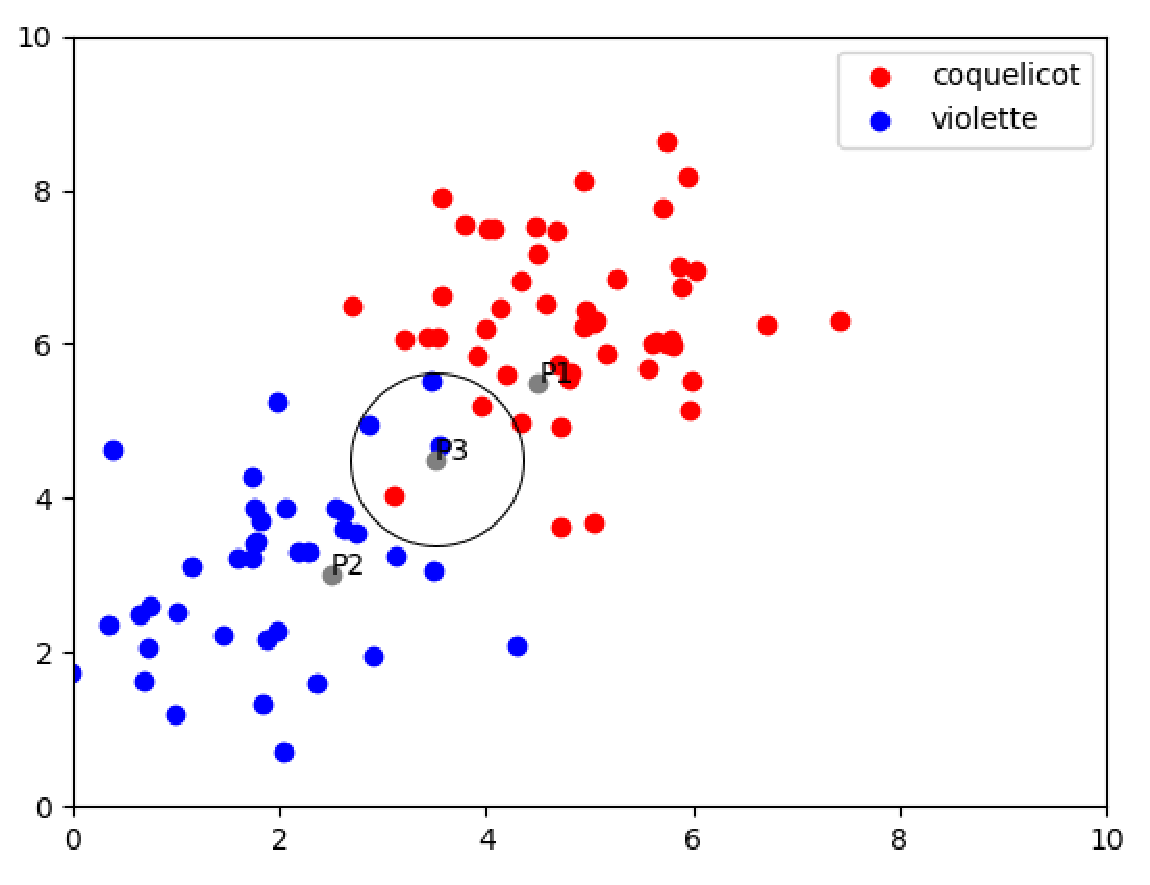
\includegraphics[height=5cm]{ex_cours3.eps}
        \end{center}
    \end{exampleblock}
\end{frame}

\makess{\textit{knn} : principe de l'algorithme}
\begin{frame}{\Ctitle}{\stitle}
	\begin{alertblock}{Principe de l'algorithme}
		\begin{itemize}
			\item<1-> L'algorithme des \textcolor{red}{$k$ plus proches voisins} est un algorithme de classification des données appartenant à la famille des algorithmes d'apprentissage \textit{supervisé}.
			\item<2-> On dispose d'un jeu de données qui associe chaque donnée à une classe.
			\item<3-> L'algorithme attribut à une nouvelle donnée $d$ non classée la classe majoritaire de ses $k$ plus proches voisins.
			\item<4-> On doit donc utiliser une distance sur l'ensemble des données (par exemple la distance euclidienne)
		\end{itemize}
	\end{alertblock}
\end{frame}


\begin{frame}{\Ctitle}{\stitle}
	\begin{exampleblock}{Exemple}
		\begin{center}
		\includegraphics[scale=0.25]{knn1.eps}
		\end{center}
		Le point gris central est la donnée à classer. Quel sera le résultat de l'algorithme :
		\begin{itemize}
			\item<2->{Pour $k=3$ ?}
			\onslide<4->{\textcolor{OliveGreen}{Il y 2 croix et un losange dans les 3 plus prochains voisins, la classe majoritaire est donc la croix et l'algorithme classe la donnée comme une croix.}}
			\item<3->{Pour $k=10$ ?}
			\onslide<5->{\textcolor{OliveGreen}{Cette fois il y a 6 losanges et 4 croix parmi les 10 plus proches voisins, la donnée est donc classée parmi les losanges.}}
		\end{itemize}
	\end{exampleblock}
\end{frame}

\makess{Matrice de confusion}
\begin{frame}{\Ctitle}{\stitle}
    \begin{block}{Test d'efficacité}
        \begin{itemize}
        \item<1-> Pour tester l'efficacité de l'algorithme, on réserve une partie des données déjà classées afin d'effectuer des tests. 
        \item<2-> Sur ces données, on peut  comparer la classe effective de la donnée avec celle fournie par l'algorithme 
        \item<3-> En particulier, le calcul de la  \textcolor{blue}{matrice de confusion}, dont le coefficient $M_{ij}$ est le nombre de données de la classe $i$ affectés à la classe $j$ permet de mesurer le taux d'erreur de l'algorithme.
        \item<4-> Ces tests permettent de déterminer une \og{} bonne \fg{} valeur de $k$
        \end{itemize}
    \end{block}
\end{frame}

\begin{frame}{\Ctitle}{\stitle}
    \begin{exampleblock}{Exemple}
        En utilisant l'algorithme des $k$ plus proches voisins pour classer des données tests on a obtenu les matrices de confusion suivantes : 
        \begin{center}
        \begin{tabularx}{\textwidth}{Y|Y}
            pour $k=4$ & pour $k=7$  \\
            $\begin{pmatrix}
                9 & 1 & 0 \\
                2 & 10 & 3 \\
                1 & 2  & 12 \\
            \end{pmatrix}$  & 
            $\begin{pmatrix}
                10 & 0 & 0 \\
                1 & 11 & 1 \\
                0 & 1  & 14 \\
            \end{pmatrix}$ \\
        \end{tabularx}
        \begin{itemize}
            \item<2-> Donner le nombre de classes, et le nombre de données tests par classe.\\
            \onslide<4->\textcolor{OliveGreen}{Il y a 3 classes, 10 données sont dans la première classe, et 15 dans chacune des deux autres.}
            \item<5-> Calculer le pourcentage d'erreur commis pour chacune des valeurs de $k$. Conclure \\
                \begin{itemize}
                    \item<7->\textcolor{OliveGreen}{Pour $k=4$, le pourcentage d'erreur est $9/40 = 22,5 \%$.}
                    \item<8->\textcolor{OliveGreen}{Pour $k=7$, le pourcentage d'erreur est $3/40 = 7,5 \%$.}
                \end{itemize}
            \onslide<9->\textcolor{OliveGreen}{La valeur $k=7$ semble être un bon choix.}
        \end{itemize}
    \end{center}

    \end{exampleblock}
\end{frame}


\begin{frame}{\Ctitle}{\stitle}
    \begin{block}{Synthèse}
        La mise en oeuvre de l'algorithme demande donc à :
        \begin{itemize}
            \item<1-> Disposer d'un jeu de données $d=(d_0, \dots d_{n-1})$ déjà classées, c'est à dire attribuées à des classes $c_0, \dots c_{m-1}$
            \item<2-> D'une distance entre deux données de façon à quantifier la notion de proximité.
            \item<3-> Choisir un nombre $k$ de voisins à considérer. La valeur de $k$ influence la prédiction de l'algorithme (voir exemple précédent). En pratique, on teste plusieurs valeurs de $k$ et on choisit celle qui donne les meilleurs résultats.
            \item<4-> Une nouvelle donnée $d_n$ est alors affectée à la classe de ses $k$ plus proches voisins.
            \item<5-> La matrice de confusion donne une appréciation de l'efficacité de l'algorithme.
        \end{itemize}
        \onslide<6->{\textcolor{blue}{Voir le TP sur les iris de Fischer pour une mise en oeuvre d'un exemple en Python.}}
    \end{block}
\end{frame}



\makess{\textit{k-moyennes} : exemple introductif}
\begin{frame}{\Ctitle}{\stitle}
    \begin{exampleblock}{Un (autre) champ de fleurs}
        Dans un champ, à l'état sauvage \textcolor{blue}{trois} espèces de fleurs ont poussées, chaque point gris indique l'emplacement d'une fleur et on souhaite prédire l'espèce de chacune des fleurs (en supposant qu'une espèce donnée pousse de façon préférentielle dans une certaine zone).
        \begin{center}
            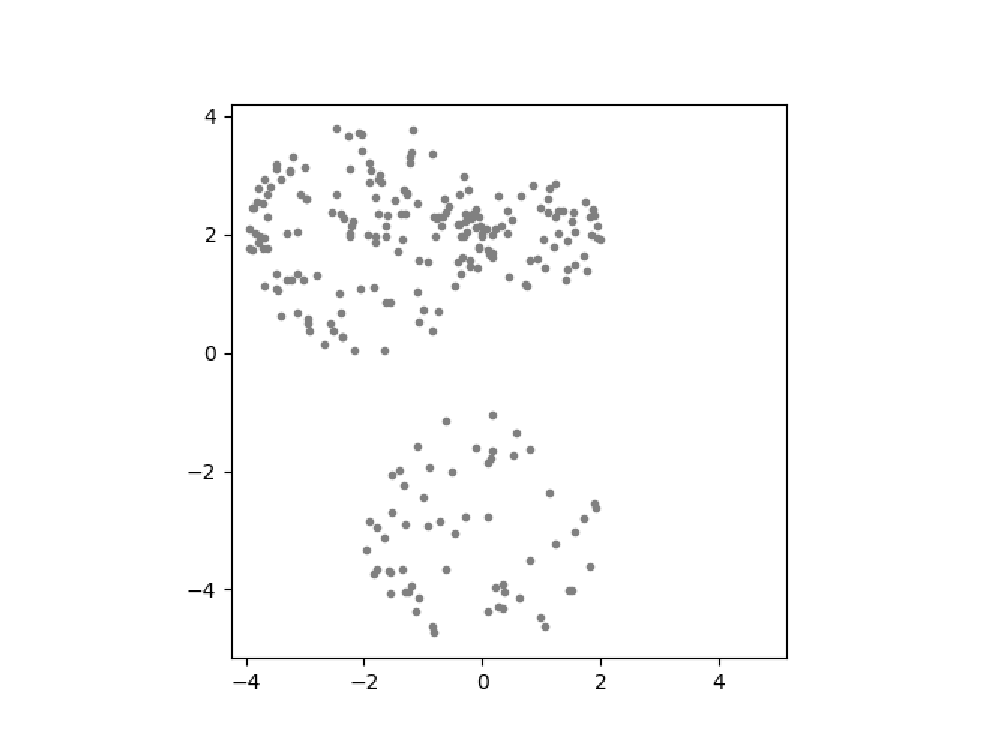
\includegraphics[height=5cm]{start_kmeans.eps}
        \end{center}
    \end{exampleblock}
\end{frame}


\begin{frame}{\Ctitle}{\stitle}
    \begin{exampleblock}{Un (autre) champ de fleurs}
        On commence par choisir \textcolor{blue}{au hasard} trois fleurs et on considère qu'elles représentent chacune des trois espèces.
        \begin{center}
            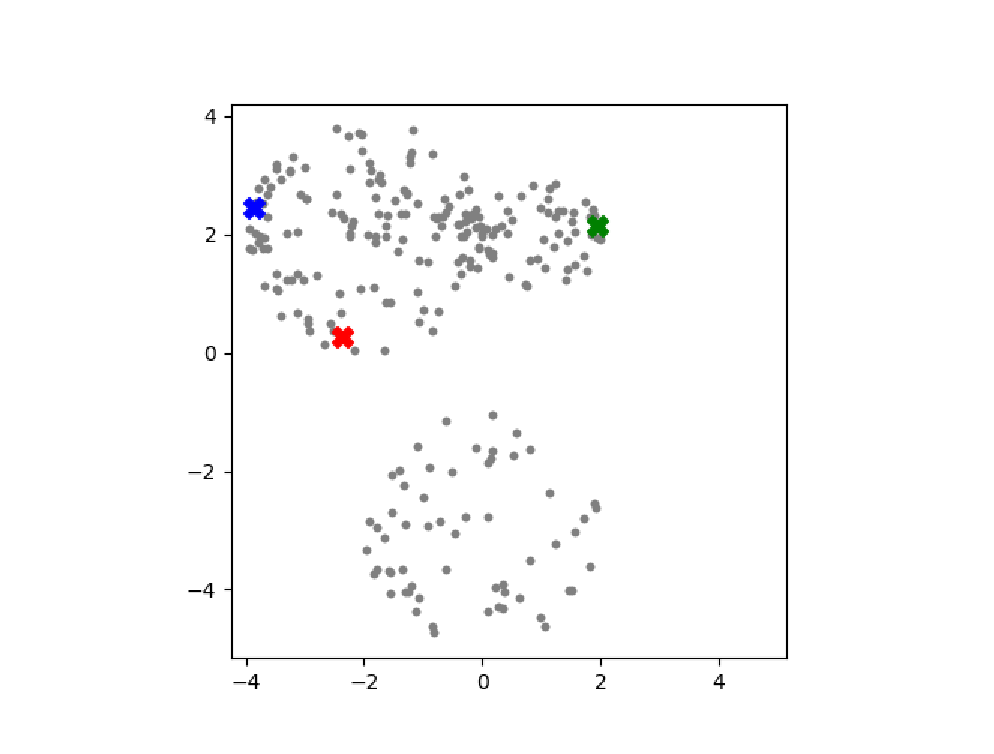
\includegraphics[height=5cm]{ex2_kmeans0.eps}
        \end{center}
    \end{exampleblock}
\end{frame}

\begin{frame}{\Ctitle}{\stitle}
    \begin{exampleblock}{Un (autre) champ de fleurs}
        On attribut alors à chaque fleur une espèce en utilisant la proximité avec les trois fleurs choisies au hasard initialement.
        \begin{center}
            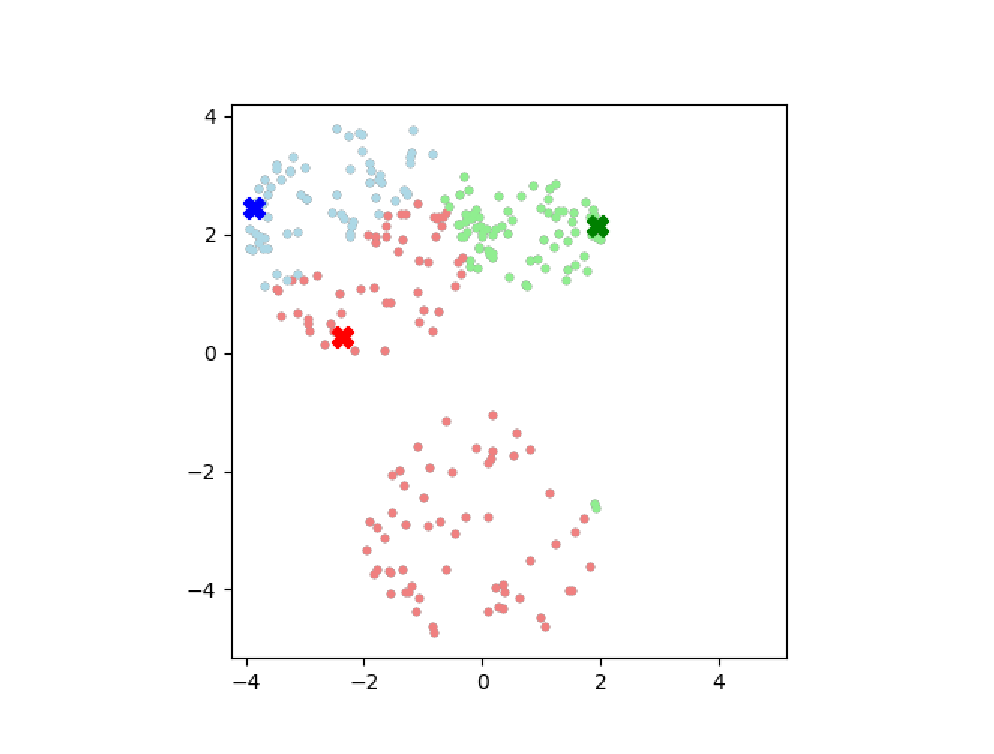
\includegraphics[height=5cm]{ex2_kmeans1.eps}
        \end{center}
    \end{exampleblock}
\end{frame}

\begin{frame}{\Ctitle}{\stitle}
    \begin{exampleblock}{Un (autre) champ de fleurs}
        Dans chaque espèce on calcule alors la position du centre du nuage de points en faisant la moyenne des fleurs appartenant à cette espèce.
        \begin{center}
            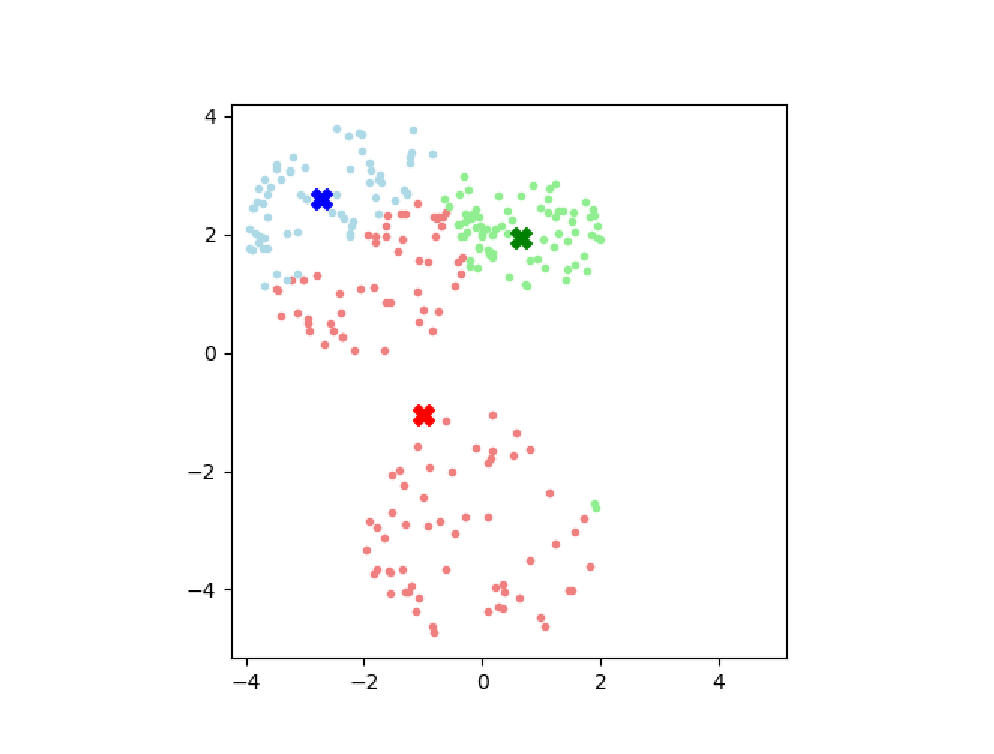
\includegraphics[height=5cm]{ex2_kmeans2.eps}
        \end{center}
    \end{exampleblock}
\end{frame}

\begin{frame}{\Ctitle}{\stitle}
    \begin{exampleblock}{Un (autre) champ de fleurs}
        Comme précédemment, on affecte de nouveau les fleurs à une espèce par rapport à leur proximité aux nouveaux centres.
        \begin{center}
            \includegraphics[height=5cm]{ex2_kmeans3.eps}
        \end{center}
    \end{exampleblock}
\end{frame}

\begin{frame}{\Ctitle}{\stitle}
    \begin{exampleblock}{Un (autre) champ de fleurs}
        On réitère les étapes précédentes : calcul des nouveaux centres puis affectation suivant la proximité.
        \begin{center}
            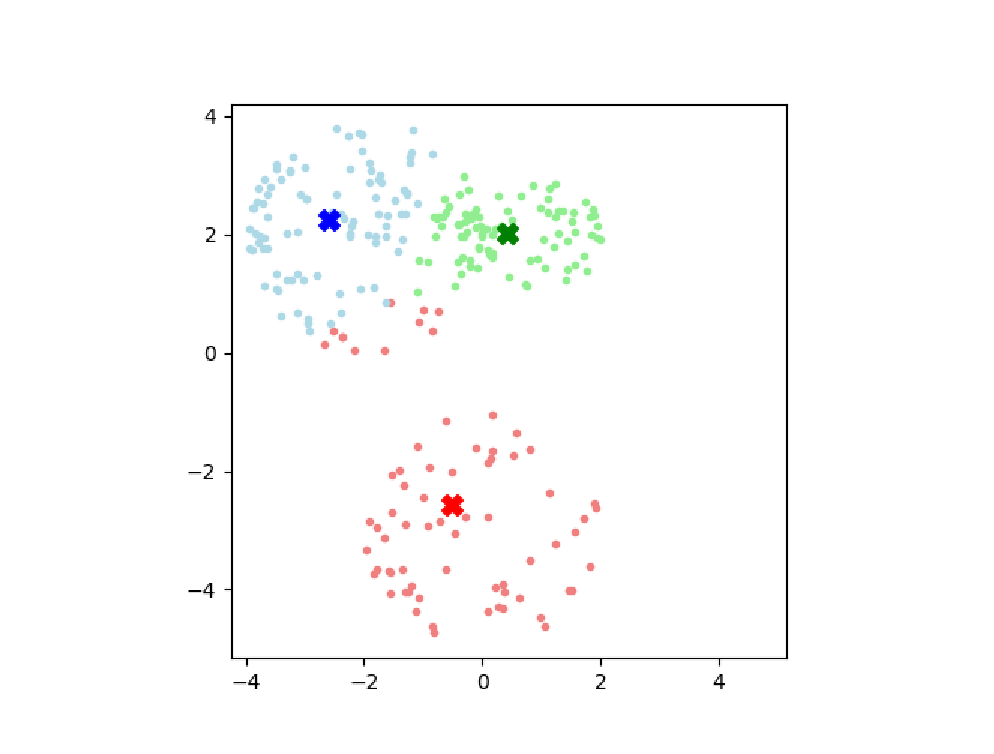
\includegraphics[height=5cm]{ex2_kmeans4.eps}
        \end{center}
    \end{exampleblock}
\end{frame}

\begin{frame}{\Ctitle}{\stitle}
    \begin{exampleblock}{Un (autre) champ de fleurs}
        On réitère les étapes précédentes : calcul des nouveaux centres puis affectation suivant la proximité.
        \begin{center}
            \includegraphics[height=5cm]{ex2_kmeans6.eps}
        \end{center}
    \end{exampleblock}
\end{frame}

\begin{frame}{\Ctitle}{\stitle}
    \begin{exampleblock}{Un (autre) champ de fleurs}
        Après un certain nombre d'étapes, la répartition se stabilise.
        \begin{center}
            \includegraphics[height=5cm]{ex2_kmeans8.eps}
        \end{center}
    \end{exampleblock}
\end{frame}

\makess{\textit{k-moyennes} : principe de l'algorithme}
\begin{frame}{\Ctitle}{\stitle}
    \begin{alertblock}{Principe de l'algorithme}
        \begin{itemize}
            \item<1-> L'algorithme des \textcolor{red}{k-moyennes} est un algorithme de classification des données appartenant à la famille des algorithmes d'apprentissage \textit{non supervisé}.
            \item<2-> Les étapes de l'algorithme sont :
            \begin{enumerate}
                \item<3-> Choisir un entier $k$ (le nombre de clusters à former) et choisir aléatoirement $k$ points de données comme centres des clusters
                \item<4-> Affecter chaque donnée au cluster dont le centre est le plus proches
                \item<5-> Mettre à jour les centres de chaque cluster en prenant comme nouveau centre la moyenne des points du cluster
                \item<6-> Répéter les étapes 2 et 3 jusqu'à atteindre un critère d'arrêt (stabilisation ou nombre maximal d'itérations)
            \end{enumerate}
            \item<7-> On montre (hors programme) que cet algorithme converge toujours.
        \end{itemize}
    \end{alertblock}
\end{frame}

\begin{frame}{\Ctitle}{\stitle}
    \begin{exampleblock}{Exemple}
        Le choix des centres initiaux influence les résultats de l'algorithme. Sur l'exemple ci-dessous on \og{} voit \fg{} bien trois cluster bien séparés contenant chacun cinq points mais ils ne seront par forcément détecté correctement.
        \begin{center}
            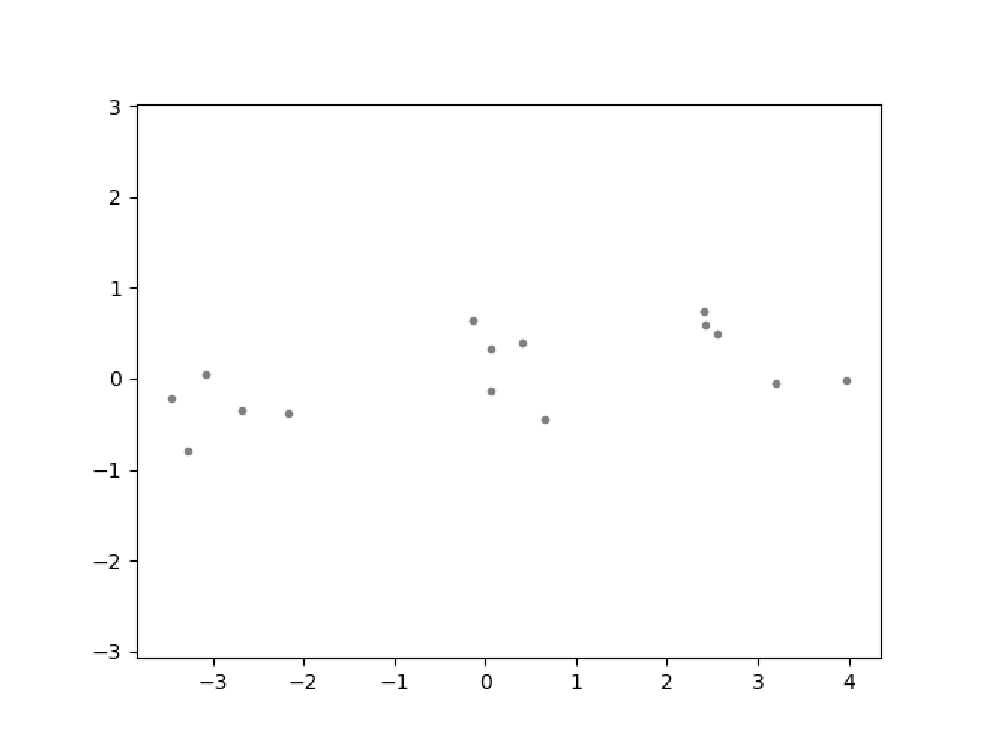
\includegraphics[height=5cm]{start_simple.eps}
        \end{center}
    \end{exampleblock}
\end{frame}

\begin{frame}{\Ctitle}{\stitle}
    \begin{exampleblock}{Exemple}
        \begin{center}
            \begin{tabularx}{\textwidth}{Y|Y}
                Centres initiaux & Résultats de la classification \\
                \includegraphics[height=4cm]{ex1_simple0.eps} & \includegraphics[height=4cm]{ex1_simple6.eps} \\
            \end{tabularx}
        \end{center}
    \end{exampleblock}
\end{frame}

\begin{frame}{\Ctitle}{\stitle}
    \begin{exampleblock}{Exemple}
        \begin{center}
            \begin{tabularx}{\textwidth}{Y|Y}
                Centres initiaux & Résultats de la classification \\
                \includegraphics[height=4cm]{ex2_simple0.eps} & \includegraphics[height=4cm]{ex2_simple4.eps} \\
            \end{tabularx}
        \end{center}
    \end{exampleblock}
\end{frame}


\end{document}